\documentclass[letterpaper,10pt]{article}

\usepackage{enumitem}
\usepackage{titling}
\usepackage{listings,listings-rust}
\usepackage{url}
\usepackage{soul}
\usepackage{hyperref}
\usepackage{setspace}
\usepackage{subfig}
\usepackage{sectsty}
\usepackage{pdfpages}
\usepackage{colortbl}
\usepackage{multirow}
\usepackage{multicol}
\usepackage{relsize}
\usepackage{amsmath}
\usepackage{wasysym}
\usepackage{fancyvrb}
\usepackage[yyyymmdd]{datetime}
\usepackage{amsmath,amssymb,amsthm,graphicx,xspace}
\usepackage[titlenotnumbered,noend,noline]{algorithm2e}
\usepackage[compact]{titlesec}
\usepackage{XCharter}
\usepackage[T1]{fontenc}
\usepackage[scaled]{beramono}
\usepackage[normalem]{ulem}
\usepackage{booktabs}
\usepackage{tikz}
\usetikzlibrary{arrows.meta,automata,shapes,trees,matrix,chains,scopes,positioning,calc,decorations.pathreplacing}
\tikzstyle{block} = [rectangle, draw, fill=blue!20, 
    text width=2.5em, text centered, rounded corners, minimum height=2em]
\tikzstyle{bw} = [rectangle, draw, fill=blue!20, 
    text width=4em, text centered, rounded corners, minimum height=2em]

\definecolor{namerow}{cmyk}{.40,.40,.40,.40}
\definecolor{namecol}{cmyk}{.40,.40,.40,.40}
\renewcommand{\dateseparator}{-}

\let\LaTeXtitle\title
\renewcommand{\title}[1]{\LaTeXtitle{\textsf{#1}}}

\lstset{basicstyle=\footnotesize\ttfamily,breaklines=true}

\newcommand{\CPP}{C\nolinebreak\hspace{-.05em}\raisebox{.4ex}{\tiny\bf +}\nolinebreak\hspace{-.10em}\raisebox{.4ex}{\tiny\bf +}}
\def\CPP{{C\nolinebreak[4]\hspace{-.05em}\raisebox{.4ex}{\tiny\bf ++}}}

\newcommand{\handout}[5]{
  \noindent
  \begin{center}
  \framebox{
    \vbox{
      \hbox to 5.78in { {\bf ECE459: Programming for Performance } \hfill #2 }
      \vspace{4mm}
      \hbox to 5.78in { {\Large \hfill #4  \hfill} }
      \vspace{2mm}
      \hbox to 5.78in { {\em #3 \hfill \today} }
    }
  }
  \end{center}
  \vspace*{4mm}
}

\newcommand{\lecture}[3]{\handout{#1}{#2}{#3}{Lecture#1}}
\newcommand{\tuple}[1]{\ensuremath{\left\langle #1 \right\rangle}\xspace}

\addtolength{\oddsidemargin}{-1.000in}
\addtolength{\evensidemargin}{-0.500in}
\addtolength{\textwidth}{2.0in}
\addtolength{\topmargin}{-1.000in}
\addtolength{\textheight}{1.75in}
\addtolength{\parskip}{\baselineskip}
\setlength{\parindent}{0in}
\renewcommand{\baselinestretch}{1.5}
\newcommand{\term}{Winter 2020}

\singlespace


\begin{document}

\lecture{20 --- Performance Case Study, Performance Culture}{\term}{Patrick Lam}

\section*{Making Firefox Fast}

Let's look at Mike Conley's Firefox Performance Updates,
\begin{center}
{\scriptsize
\vspace*{-1em}
\url{https://mikeconley.ca/blog/2018/02/14/firefox-performance-update-1/}
}
\end{center}
\vspace*{-1em}

\begin{itemize}[noitemsep]
\item don't use CPU animating out-of-view elements
\item move db init off main thread
\item keep better profiling data
\item parallel painting for macOS
\item lazily instantiate Search Service only when first search starts
\item halve size of the blocklist
\item refactor to reduce main-thread IO
\item don't hold all frames of animated GIFs/APNGs in memory
\item eliminate an unnecessary hash table
\item use more modern compiler
\end{itemize}

We can categorize most of these updates into the categories we've seen before:
\begin{itemize}[noitemsep]
\item do less work\\
 (or do it sooner/later);
\item use threads (move work off main thread);
\item track performance;
\end{itemize}
Which of the updates fall into which categories?

\subsection*{Tab warming} We continue by examining one particular update, \emph{tab warming}, in detail:
\begin{center}
\scriptsize
\vspace*{-1em}
\url{https://mikeconley.ca/blog/2018/01/11/making-tab-switching-faster-in-firefox-with-tab-warming/}.
\end{center}
\vspace*{-1em}

\hfill ``Maybe this is my Canadian-ness showing, but I like to think of it almost like coming in from shoveling snow off of the driveway, and somebody inside has \emph{already made hot chocolate for you}, because they knew you’d probably be cold.'' --- Mike Conley

Consider switching tabs. Previously, Firefox would request a paint of the newly-selected tab and wait for the rendering to be available before switching the tab.

The idea is to reduce user-visible latency by predicting an imminent tab switch. How do you know that the user is about to switch tabs? When the user has a mouse, then the mouse cursor will hover over the next tab.

\begin{quote}
Assuming a sufficiently long delay between hover and click, the tab switch should be perceived as instantaneous. If the delay was non-zero but still not long enough, we will have nonetheless shaved that time off in eventually presenting the tab to you.

And in the event that we were wrong, and you weren’t interested in seeing the tab, we eventually throw the uploaded layers away.
\end{quote}

The blog post does not report performance numbers (but bug 1430160 discusses how to collect them).

\subsection*{Firefox in general}

Try: ``about:mozilla'' in Firefox. On a Quantum Flow-enabled version, you'll see

\begin{center}
\emph{The Beast adopted new raiment and studied the ways of Time and Space and Light and the Flow of energy through the Universe. From its studies, the Beast fashioned new structures from oxidised metal and proclaimed their glories. And the Beast’s followers rejoiced, finding renewed purpose in these teachings.}

\hfill \emph{from The Book of Mozilla, 11:14}
\end{center}

In 2017, Mozilla released Electrolysis (E10s)~\cite{electrolysis}.
which leverages multicore processors by using multiple OS-level
processes. (Chrome has always done this, but Firefox attempts to also
keep memory usage
down~\cite{goldilocks}.
Beyond internal architecture issues, handling Add-Ons (now
WebExtensions) was perhaps the most challenging part of going
multi-process.

Note the connection to different thread/process models.
Chrome is one-process-per-tab, while Firefox multiplexes tabs across
the 4 content processes (``hardware threads'', by analogy). Limiting
the number of tabs also limits the memory consumption of the browser:
we don't have arbitrary numbers of renderer state.

\begin{center}
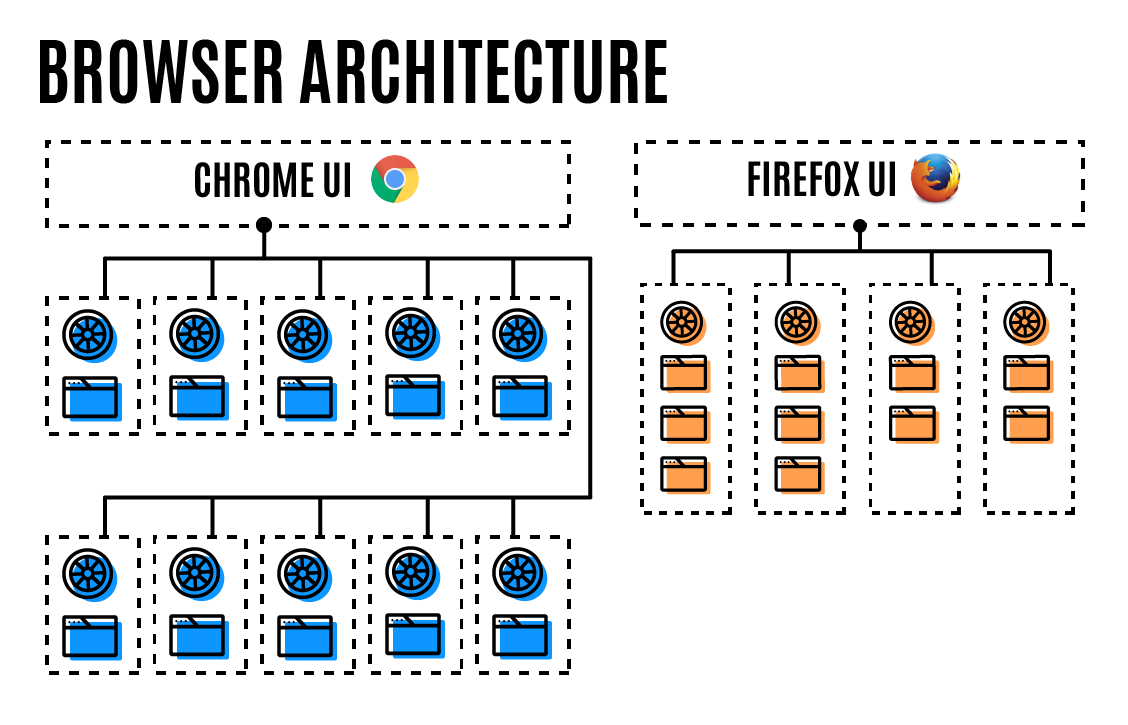
\includegraphics[width=.9\textwidth]{images/L19-chrome-vs-firefox.png}
\end{center}
Source: Ryan Pollock~\cite{goldilocks}

As a crude summary, Electrolysis works on splitting across processes
while the newer Quantum Flow leverages multithreading and other
improvements.  Quantum Flow uses the Rust programming language and its
``fearless concurrency'' (in Rust-speak). Rust should probably be part
of a future revision of the ECE 459 curriculum. But we'll focus on
Firefox here.

\subsection*{Quantum Flow}
Here's a retrospective of the Quantum Flow project:
\begin{center}
\url{https://ehsanakhgari.org/blog/2017-09-21/quantum-flow-engineering-newsletter-25}
\end{center}

To sum up, they formed a small team and did the following.
\begin{enumerate}[noitemsep]
\item Measure slowness: gather information, instrument Firefox, collect profiling data and measurements. Prioritize issues.
\item Gather help: convince other teams to pitch in with perf improvements. Examples: front-end team (reduce flushes, timers); layout team (reflow performance).
\item Fix all the things! (Or at least the most important ones).
\end{enumerate}
Given the short timeline they gave themselves (6 months) and the limited resources, an important part of their work was convincing others to help.
They triaged 895 bugs and fixed 369 of them. The weekly Quantum Flow Engineering Newsletter was a key motivational tool.

After the project wound down, they aimed to distribute responsibility for perf improvements across the entire project.

\section*{Firefox Telemetry}
Firefox's Telemetry feature collects lots of information from Firefox
users.  Idea: collect data before hacking away at things.  Firefox collects hundreds of
gigabytes of anonymous metrics per day while browsing and makes it all available to
the public.  One can view this as an analogy of CPU profiling on a
massively distributed context. This data is collected much less often than
CPU profiling data but at a much broader scope.
\begin{center}
\url{https://telemetry.mozilla.org/}
\end{center}
If you are running Firefox and want to see what it is collecting:
\begin{center}
\url{about:telemetry}
\end{center}

You can view distributions of telemetry probes (in the form of
histograms). You can also make your own dashboard based on Firefox
Telemetry data and Mozilla has infrastructure for their developres to
formulate and evaluate their own queries.

Example questions:
\begin{itemize}[noitemsep]
\item Is Firefox the user's default browser? (69\% yes)
\item Does e10s make startup faster? (no, slower)
\item Which plugins tend to freeze the browser on load? (Silverlight and Flash)
\end{itemize}
Can see evolution of data over time.

Firefox developers can propose new telemetry probes which are reviewed
for data privacy\footnote{Mozilla Data Collection Practices: \url{https://wiki.mozilla.org/Firefox/Data_Collection}} as well as through normal code review channels.

\paragraph{Pings.} Firefox phones the data home using so-called ``pings''.
Firefox sends a ``main ping'' every 24 hours, upon shutdown, environment change,
and crash. There are other types of pings as well. Pings get sent either by Firefox
or by a helper program, Pingsender, when Firefox isn't running. Presumably they
are sent over the network as compressed JSON to a central server.

Here's the common ping structure:

\begin{verbatim}
{
  type: <string>, // "main", "activation", "optout", "saved-session", ...
  id: <UUID>, // a UUID that identifies this ping
  creationDate: <ISO date>, // the date the ping was generated
  version: <number>, // the version of the ping format, currently 4

  application: {
    architecture: <string>, // build architecture, e.g. x86
    buildId: <string>, // "20141126041045"
    name: <string>, // "Firefox"
    version: <string>, // "35.0"
    displayVersion: <string>, // "35.0b3"
    vendor: <string>, // "Mozilla"
    platformVersion: <string>, // "35.0"
    xpcomAbi: <string>, // e.g. "x86-msvc"
    channel: <string>, // "beta"
  },

  clientId: <UUID>, // optional
  environment: { ... }, // optional, not all pings contain the environment
  payload: { ... }, // the actual payload data for this ping type
}
\end{verbatim}

Pings contain scalars (counts, booleans, strings) and histograms. A histogram collects
bucketed data (think grade distributions). Both scalars and histograms can be keyed, e.g.
how often searches happen for which search engines.

\section*{Laws of Performant Software}

Suppose you want to write fast programs and you like checklists and handy rules. If so, you are in luck, because there is Crista's Five Laws of Performant Software~\cite{lpsw}. 

\paragraph{1. Programming language $<<$ Programmers' awareness of performance.}
There is no programming language that is magic, whether good or evil. All the major programming languages allow you to write programs that perform well or badly. 

There's a lot of C-elitism in the world, and then there's the back-in-my-day-sonny people who claim assembly was best, and they also had to walk to school in the snow, uphill both ways.  High level languages give you lots of options... Do I use an array? A vector? A list? And yes, some of the fancy tools you get are syntactic sugar: they are convenient from the programmer's point of view, but what do they do behind the scenes? If the performance is not what you expect, there is probably be a better way to do it in the high level language.

I'll add my own asterisk on this rule: some languages lend themselves better to parallelization than others. A language may force a certain way of thinking, based on its rules (e.g., functional programming languages). But there is no reason why the way of thinking can't be applied in another language.


\paragraph{2. $d(f^{\tau}(x), f^{\tau}(y)) > e^{\alpha\tau} d(x, y)$ or small details matter.} This complicated formula is from the butterfly effect (chaos theory). If two versions of the code are $x$ and $y$, the difference between the performance outcomes $f(x), f(y)$ is much larger than the difference between the code.

A small code change can have a huge impact. Did you fix a memory leak? The addition of one \texttt{free()} call is a single line code change but can, in the long run, have a dramatic impact on performance. Is caching used properly? Can you use a faster serialization algorithm? 

Basically: don't overlook the small stuff. It's tempting to think that huge major architectural changes are the solution to everything; but there are plenty of gains to be found in the small things.

\paragraph{3. corr(performance degradation, unbounded resource usage) > 0.9.}
There is a very high correlation between performance degradation and unbounded use of resources. Often times we focus on functionality: the software must have the following 847~251 features! But if you want a program that scales you need to think in terms of operation, not functionality.

Resources need to be limited. If there aren't hard limits, eventually a resource will be exhausted. If the program starts threads, use a thread pool and the thread pool should have a fixed size. Is there a cache? It needs a maximum size. If you need to read input, don't use a function that reads an entire line (of arbitrary length). Furthermore your program needs design effort given to what happens when resources are exceeded. So you decide to set a request queue size; once that queue is full, further requests are rejected in some well-understood manner. 

\paragraph{4. Performance improvements = log(controlled experiments)}
If you want your code to be faster you have to know why it is slow. It's okay not to know the answers, but not knowing how to find out is a problem. Don't guess; measure.


\paragraph{5. N*bad != good.}
No amount of nodes, cores, memory, etc, will save you from poorly-written code. Throwing more hardware at the problem is expensive and ineffective in the long term. Bad code is still bad no matter how much hardware it runs on. 

\section*{Performance Tips}

While we're on the soapbox, a few more small things to note from~\cite{preopt} about how one might write code in a performant as well as maintainable way.

\paragraph{Understand the order of magnitude that matters.} If you are writing code where 100 CPU cycles matters, then a function that will acquire a lock through some sort of shared-memory interlocked instruction then this instruction is performance murder. And it might be even worse if lock acquisition fails and you get blocked for 100~000 cycles trying to acquire the lock... On the other hand, if you have a network intensive then the 100 cycle stuff does not matter even the smallest bit because it is lost in the noise of the network.

\paragraph{Plan for the worst case scenario.} I don't mean for the nuclear apocalypse, as much fun as that might be. As~\cite{preopt} wrote:

\begin{quote}
What happens if that lock is held for longer than expected, because the system is under load and the scheduler is overloaded? And what if the owning thread was preempted while holding the lock, and now will not get to run again for quite some time? What happens if the network is saturated because a big news event is underway, or worse, the phone network is intermittently cutting out, the network cable has been unplugged, etc.? What about the case where, because a user has launched far too many applications at once, your memory-intensive operation that usually enjoys nice warmth and locality suddenly begins waiting for the disk on the majority of its memory accesses, due to demand paging? These things happen all the time.

In each of these situations, you can end up paying many more orders of magnitude in cost than you expected under ordinary circumstances. The lock acquisition that usually took 100 CPU cycles now takes several million cycles (as long as a network roundtrip), and the network operation that is usually measured in milliseconds is now measured in tens of seconds, as the software painfully waits for the operation to time out. And your ``non-blocking'' memory-intensive algorithm on the UI thread just caused a hang, because it's paging like crazy.
\end{quote}

No doubt you have seen these sorts of things as well and it is an awful user experience. The spinning beach ball of death and the ``Not Responding'' added to the title bar are all symptoms of this situation. 

\paragraph{Acknowledge and plan for asynchrony.} A quick example from~\cite{preopt}: suppose that Jordan is writing code to return a list of fonts to be used in the UI. The code checks a local font cache, and if that is already initialized, returns the fonts found in the cache in a List object. If the cache is not initialized, however, the data needs to be loaded, perhaps from the printer (which will dutifully tell you what fonts it can print out). Morgan intends to use this list of fonts in the UI of the program but is unaware that in certain circumstances this call will take much longer (that is, when the cache is not initialized).

Supposing that the API just returns a \texttt{List<Font>}, it is not obvious to Morgan where these come from. And in local testing on the dev machine with nothing on it and nothing else doing and the printer is always turned on, and rainbows and unicorns are present. Thus even if the cache is not initialized it is ``fast enough''. But in the real world, of course, the printer will be down and unicorns are nowhere to be found and it runs up against some hard timeout of 20 seconds. 

If, however, Jordan's API now has a return type of \texttt{Task<List>} (generify as desired), then it is obvious to Morgan that there is something asynchronous going on here at least some of the time. With this information in hand, the UI won't wait for this task and we might even convince Jordan to give us partial results (so we can draw the UI elements as backing data arrives) or at the very least, a progress bar. Users love progress bars. They are wildly inaccurate and not super informative even if they are accurate, but at least they give the user the impression that something is happening.

That actually leads us down a side debate about how to make the program appear faster than it is by some UI trickery and psychological ``hacks'', but that is beyond what we want to talk about here...

\section*{Performance Culture}

Now let's take it up a level: how do you make performance an important aspect of the culture of development of a project. The source for this section is~\cite{perfculture}.

The author's recommendations of warning signs that performance culture is off the rails:

\begin{itemize}
\item Answering the question, ``how is the product doing on my key performance metrics,'' is difficult.
\item Performance often regresses and team members either don't know, don't care, or find out too late to act.
\item Blame is one of the most common responses to performance problems (either people, infrastructure, or both).
\item Performance tests swing wildly, cannot be trusted, and are generally ignored by most of the team.
\item Performance is something one, or a few, individuals are meant to keep an eye on, instead of the whole team.
\item Performance issues in production are common, and require ugly scrambles to address (and/or cannot be reproduced).
\end{itemize}

As tempting as it is to say these are all technical issues, they are really human problems. It would obviously be preferable to start with a good performance culture in the first place, but that is not always going to happen. But suppose you are already in a hole. The usual course of action is to stop and say to yourself ``I appear to be in a hole... I know, I'll dig my way out!''. Maybe I am cynical. The right thing to do would be stop digging, of course...

Change has to come from both the top down and the bottom up. Management needs to make performance a priority: ask questions, demand rigour... while at the same time, people doing the development need to understand the performance of what they write, making practice improvements. Both sides need to have zero tolerance for regression.

If only one person is responsible for performance, this will not work. One person could not reasonably keep up with the rest of the team. If the other developers don't have performance in mind when writing, it would mean the key performance person would spend unnecessary time rewriting things when the it could have been right in the first place. If this isn't convincing, think about unit tests. Could you really ``outsource'' the writing of all unit tests to one person? And would code quality be the same if you did?

The author is very adamant that poor performance culture is management's fault. Managers need to budget time, reward the work, and encourage performance work. Managers who don't understand performance culture are likely to be caught by surprise and blame things. 

Consider the following comparison from~\cite{perfculture}:

\begin{quote}
Manager A gives lip service to performance culture. She, however, packs every sprint schedule with a steady stream of features -- ``we've got to crush competitor Z and must reach feature parity!'' -- with no time for breaks in-between. She spends all-hands team meetings praising new features, demos aplenty, and even gives out a reward to an engineer at each one for ``the most groundbreaking feature.'' As a result, her team cranks out features at an impressive clip, delivers fresh demos to the board every single time, and gives the sales team plenty of ammo to pursue new leads. There aren't performance gates and engineers generally don't bother to think much about it.

Manager B takes a more balanced approach. She believes that given the competitive landscape, and the need to impress customers and board members with whizbang demos, new features need to keep coming. But she is also wary of building up too much debt in areas like performance, reliability, and quality for areas she expects to stick. So she intentionally puts her foot on the brake and pushes the team just as hard on these areas as she does features. She demands good engineering systems and live flighting of new features with performance telemetry built-in, for example. This requires that she hold board members and product managers at bay, which is definitely unpopular and difficult. In addition to a reward for ``the most groundbreaking feature'' award at each all-hands, she shows charts of performance progress and delivers a ``performance ninja'' award too, to the engineer who delivered the most impactful performance improvement. Note that engineering systems improvements also qualify!
\end{quote}

But this is a startup, you object, why does it matter, because we need the minimum viable product and we needed it yesterday, and also, VCs like features. Well maybe, but architecture matters. There's time to fix things later, maybe, but you can really cripple your startup by choosing the wrong things early on. 

After a discussion of the why and the what, it is time to think about how to make it systematic. If it is not systematic, it will not get done and it will be dropped when in a time crunch. And development teams are always in a time crunch! This is why best practices have automated unit tests that run on every commit (or at least build). And much the same way, there need to be performance tests; if something has significantly regressed performance, the build failed and the commit is no good. This obviously requires that the tests be meaningful, testing effectively and not overly noisy. 

Performance tests may be a bit too large and difficult to run for every commit or every build. Although it would be nice to know exactly which commit is the cause of the problem, you may want a test that runs overnight to see the long term trends. And thus a 12-hour test is probably unsuitable for this. The solution is, obviously, levels of test. 

One company I worked for did something like this, although it was not performance specific. Before committing to the cvs repository (at this point nobody had heard of git  and it was the newest thing) there was a set of tests called ``precheckin''. Nobody forced a developer to run it, but you were definitely supposed to, and it just verified that everything would compile and some basic stuff worked. These tests took a few minutes to run. Then each build on the build server had a larger set of tests (``build''), including the precheckin material and a lot more, taking about 30-40 minutes to execute. Breaking this breaks the build (and gets everyone's attention). Then there were the ``regression'' tests that ran overnight (and ALL night).

In~\cite{perfculture} a zero tolerance rules advocated: anything that significantly regresses performance is reverted and re-worked. No exceptions, no questions, no pleading one's case, etc. If exceptions are allowed, exceptions quickly become the rule, and promises to fix something later are procrastinated endlessly.

Obviously when code does more it should be expected to take longer, but then the test(s) should be adjusted as well. This is the same as when developing new features/changes, after all; unit tests are adjusted when code changes are introduced intentionally.

\paragraph{Metrics} There are, roughly speaking, two categories of metrics:

\begin{itemize}
	\item \textit{Consumption}: measure resources consumed by running a test.
	\item \textit{Observational}: measure the outcomes of running the test, from the view of outside the system.
\end{itemize}

Consumption metrics are the things that we can easily measure about the code run during the test: cache misses, TLB misses, context switches, number of I/Os, memory allocated, number of system calls (traps are interrupts, remember). Observational metrics are more along the lines of time it takes to run a dataset, or number of work items processed per unit time, etc.

It might seem like observational metrics are all that we care about. End users care about the amount of time it takes to complete their work, or management/sales/marketing/C-levels care about the throughput and that's it. This matters, sure, but it's not enough to know the outcome; the consumption metrics are necessary to break down why the total time (or throughput) is what it is.

Suppose a change is committed and the tests run and the total time it takes increases by 10\%. If that's all you know, you know that things got worse but have no data as to why. You can obviously read the source code or the diff and try to look for it, but even that might not tell you enough. If you see that memory allocations are reported and you have now allocated more memory than before,  at least you have a theory to start with on what's slowing down the code. It might not be that, it might be something else entirely, but it's a place to start. Memory allocation changes are relatively easy to spot though: there's a new call to \texttt{malloc} or a structure has been extended in some way. If it is a cache miss issue, finding that without the data is harder...

Does this remind you of \texttt{printf} debugging? It's a little bit like that. But then again, you want to use this sort of thing for long running tests anyway. If the test is going to run for 4h it would be helpful to know where exactly in that four hours it went off the rails (on a crazy train!). 

There's one more consideration and that is the variability between runs. In the ideal situation, there is consistent performance every run. That is probably too much to ask for and there will be some natural variation due to nondeterminism in computers. But a change that causes a wild change in the variance is also no good; a test that sometimes finishes in 0.5$x$ time and sometimes in 2$x$ time has a high variance and this will not be acceptable. 

Be ready to dig deep: suppose a developer has introduced a change that is slow under rare circumstances. Those rare circumstances are not triggered until $n$ years later when a second developer introduces another change. The second change will be identified, at least initially, as the ``problem''. There's two ways to go about it; either fix the initial change or work around it. Which one is correct will depend very much on the circumstances, but at the very least both options should be considered. It's not about blame or not about fault; it's about improving the performance of the software.


\bibliographystyle{alphaurl}
\bibliography{459}


\end{document}
